% This is a LaTeX file. It is a text file that is compiled
% by a program called LaTeX into a pretty PDF file.
% If you're viewing this file in Overleaf, you'll see that PDF
% in the window to the right.
%
% This file is for typesetting YOUR ANSWERS to this homework assignment.
% The LaTeX macro language is complicated, so we have inserted lots of
% documenting comments into the file. Comments start with '%'
% and continue to the end of the line. In Overleaf's edit window, they
% are colored green.
%
% Comments prefixed with 'Student:' are relevant to students. Skip any-
% thing else you don't understand, or ask me.

\documentclass{article}
%% This is some font management depending on the TeX “engine” being used.
%% Nothing to worry about.
\usepackage{ifxetex}
\ifxetex
  \usepackage{fontspec}
\else
  \usepackage[T1]{fontenc}
  \usepackage[utf8]{inputenc}
  \usepackage{lmodern}
\fi

%% Student: These lines describe some document metadata.
\title{Problem Set 3}
\usepackage{etoolbox}
\makeatletter\preto{\@title}{Answers to }\makeatother
\author{%
%% Student: change the next line to your name!
    Hongyi Zheng
\\  CSCI-UA 310 Basic Algorithms
}

%% These lines set up the question, answer, and solution environments.
\usepackage{amsthm}
\usepackage{amssymb}
\theoremstyle{plain}
\newtheorem{question}{Question}

\newenvironment{answer}[1][Answer]
    {\begin{proof}[#1]{$ $}\renewcommand\qedsymbol{$\vartriangle$}}
    {\end{proof}}
\newenvironment{solution}[1][Solution]
    {\begin{proof}[#1]{$ $}\renewcommand\qedsymbol{$\blacktriangleup$}}
    {\end{proof}}
\makeatletter
    \newcommand{\stepenumdepth}{\advance\@enumdepth\@ne}
\makeatother
\AtBeginEnvironment{question}{\stepenumdepth}
\AtBeginEnvironment{answer}{\stepenumdepth}
\AtBeginEnvironment{solution}{\stepenumdepth}

\usepackage{amsmath}
\usepackage{siunitx}
\DeclareSIUnit{\pound}{lb}
\usepackage{bm}

\usepackage{tikz}
\usetikzlibrary{calc}
\usepackage{caption,subcaption}

\usepackage{hyperref}
\usepackage{graphicx}
\usepackage{enumerate}
%% This is the beginning of the part of the file that describes
%% the actual text of the document.
%% That's why it says `\begin{document}' below. :-)
\begin{document}
\maketitle


\begin{question}
\end{question}
%% Student: put your answer between the next two lines.
\begin{answer}
    \begin{enumerate}
        \item
        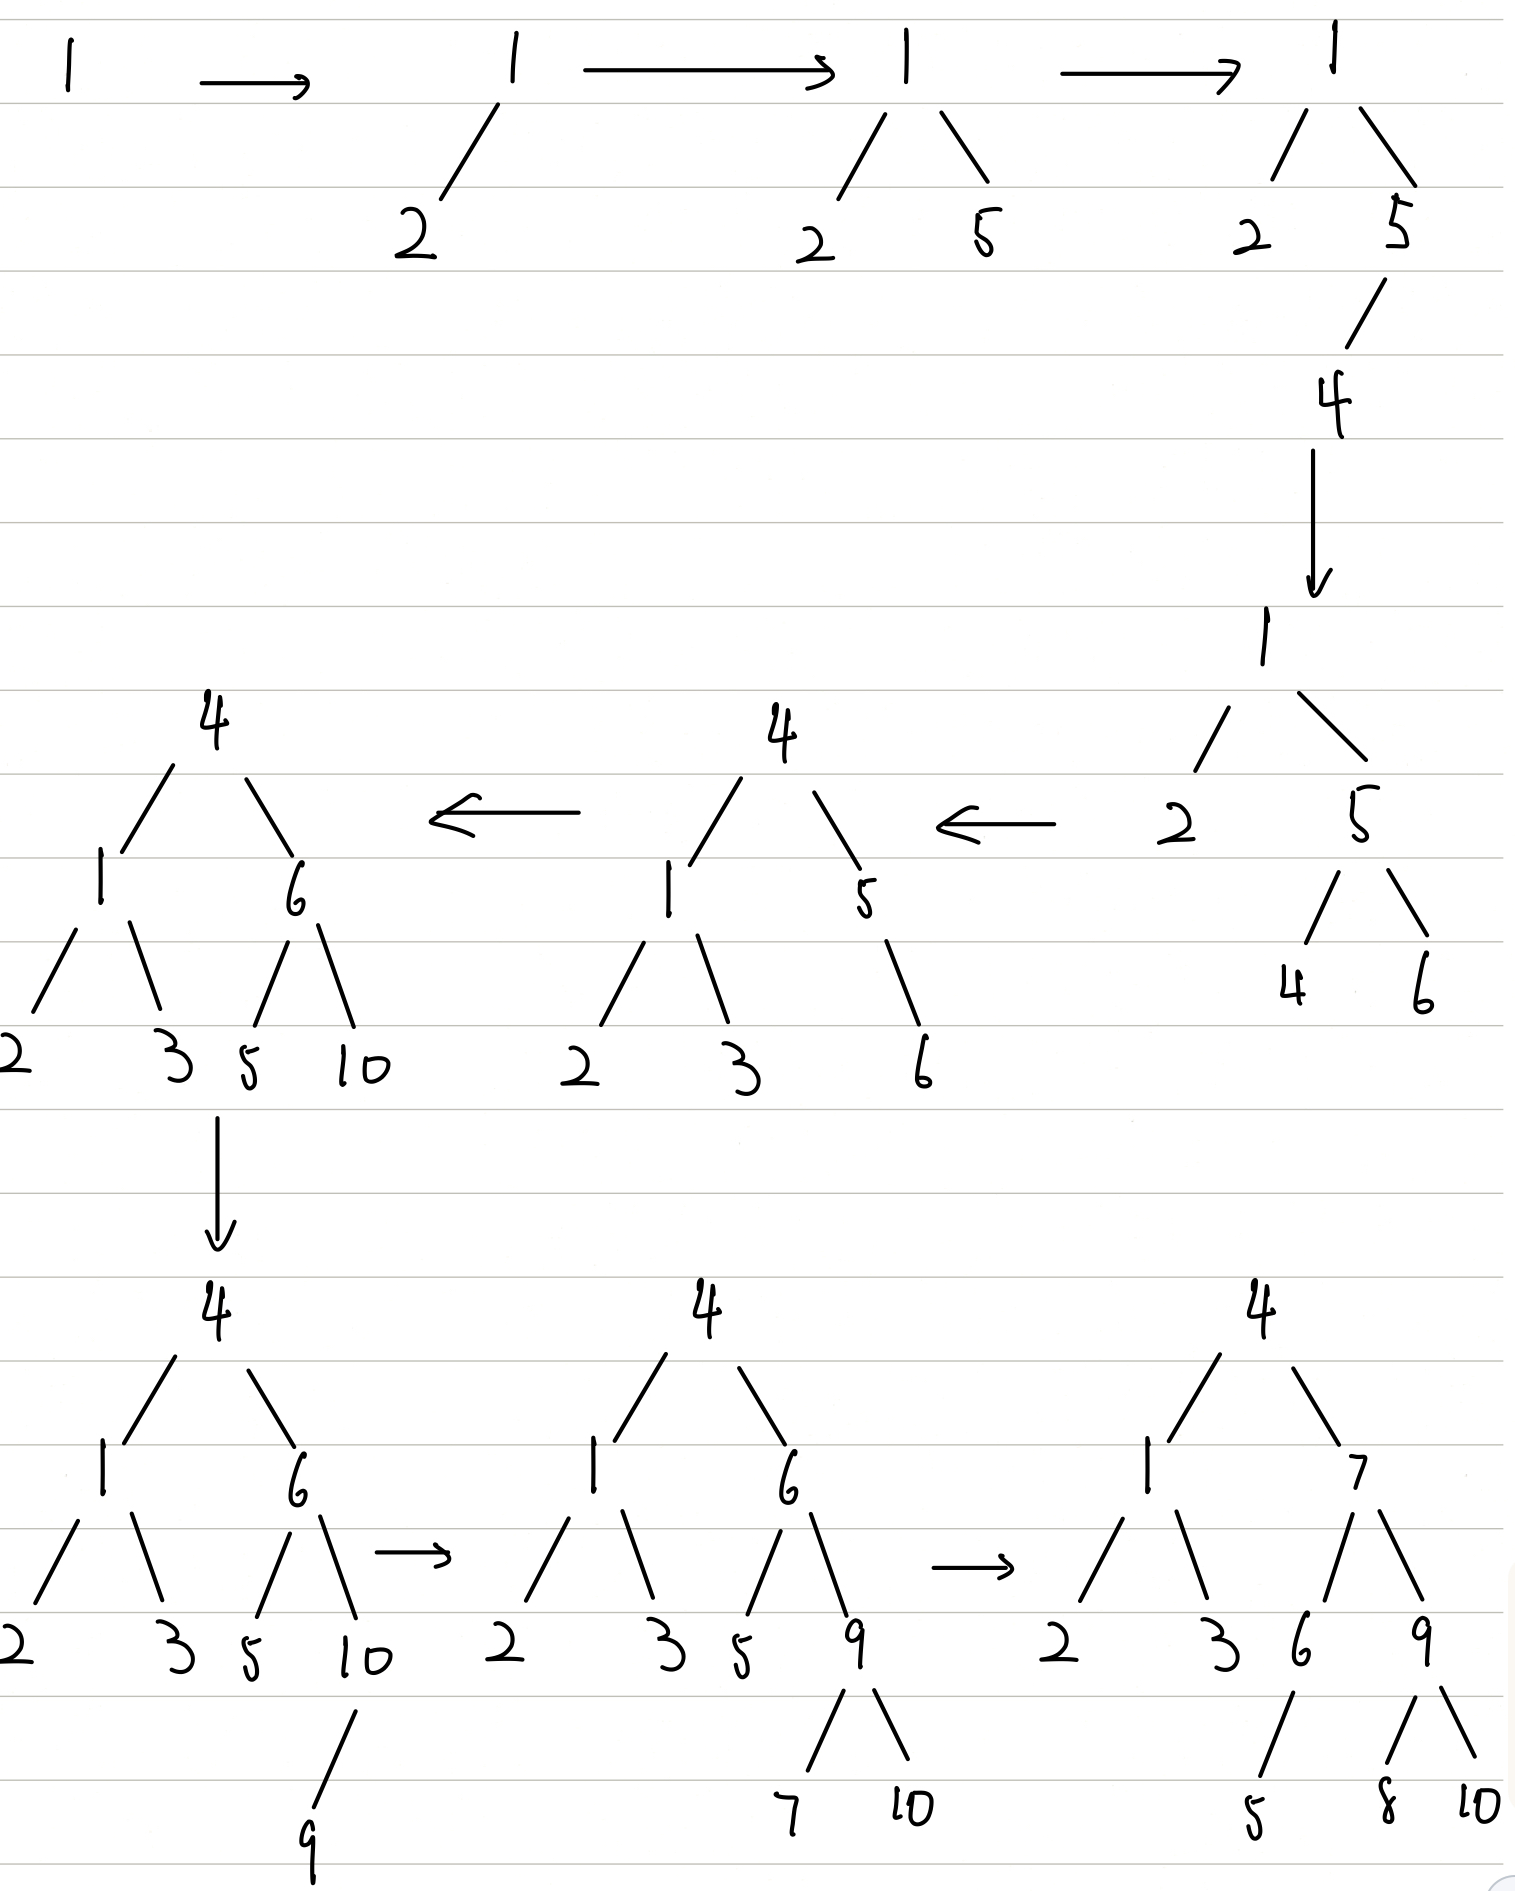
\includegraphics[width=0.8\columnwidth]{Q1_1.jpg}
        \item
        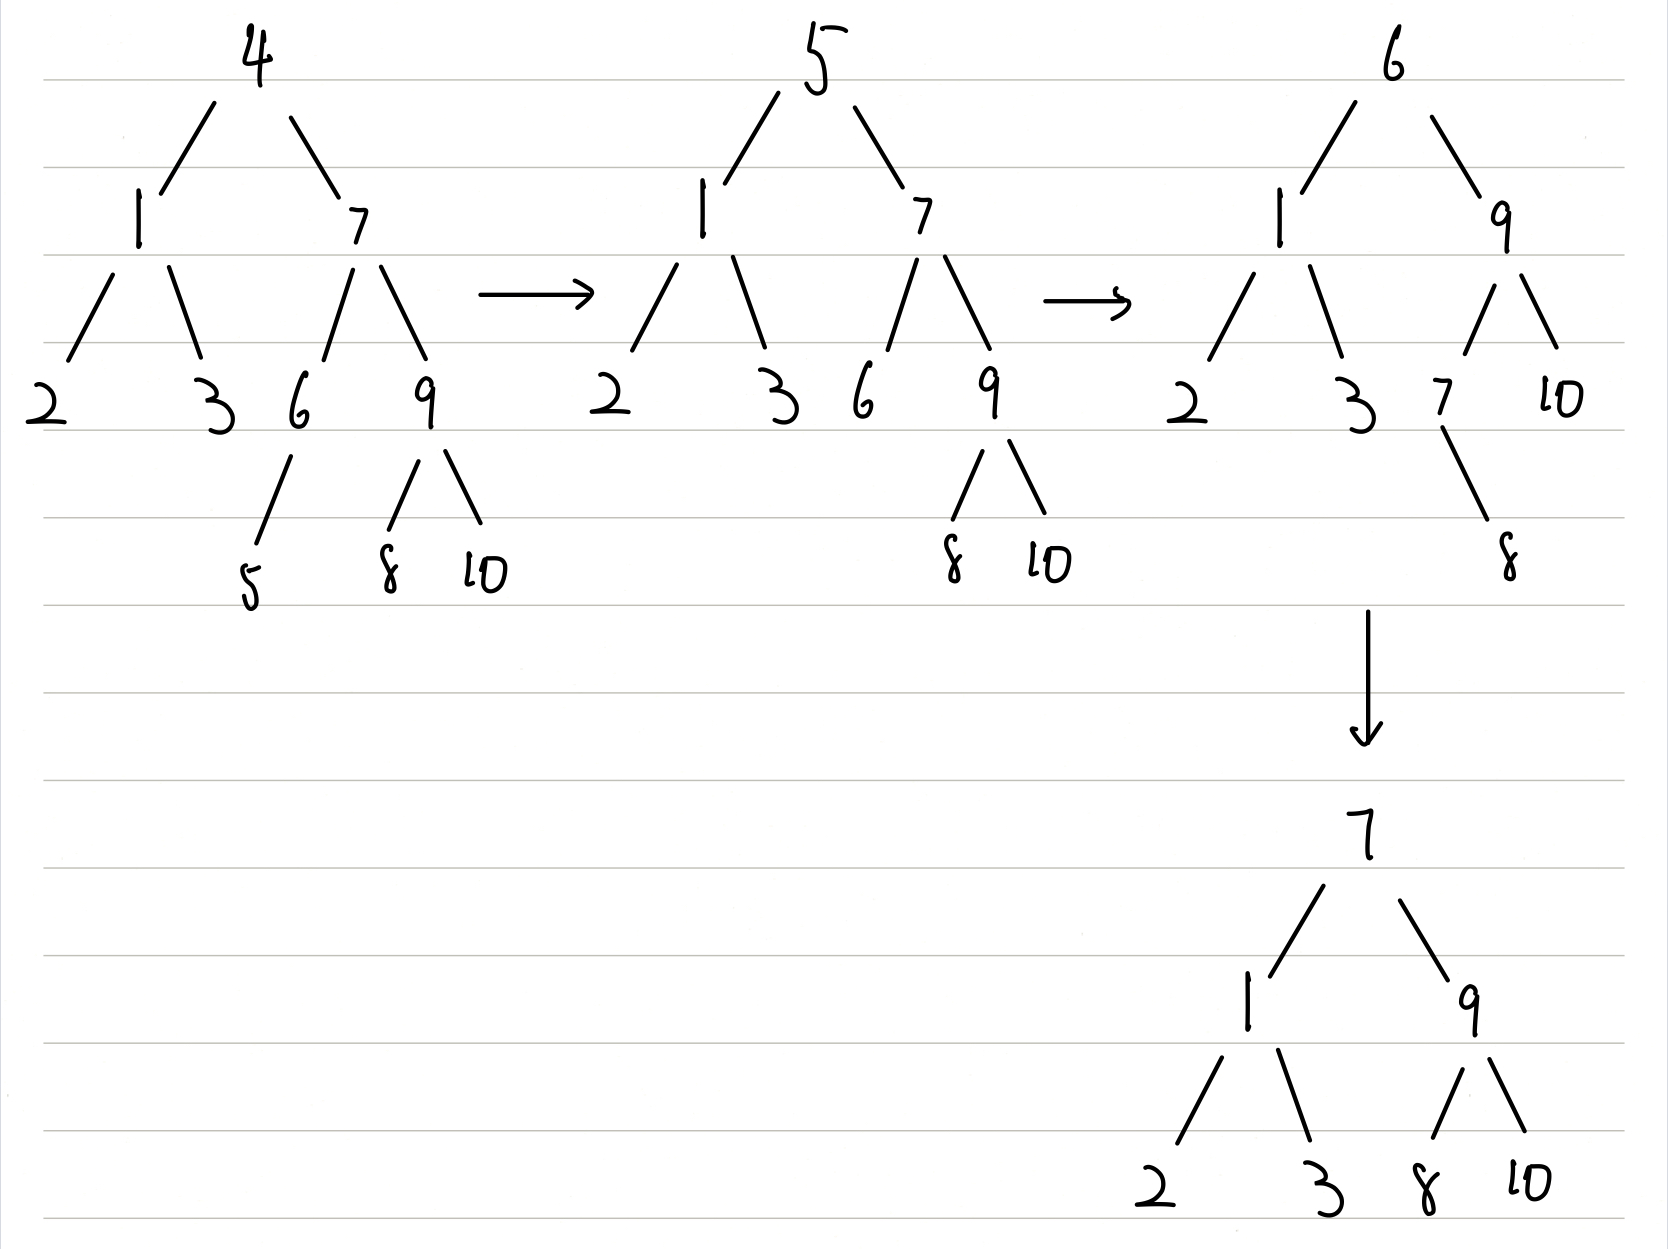
\includegraphics[width=0.9\columnwidth]{Q1_2.jpg}
    \end{enumerate}
\end{answer}

\begin{question}
\end{question}
\begin{answer}
    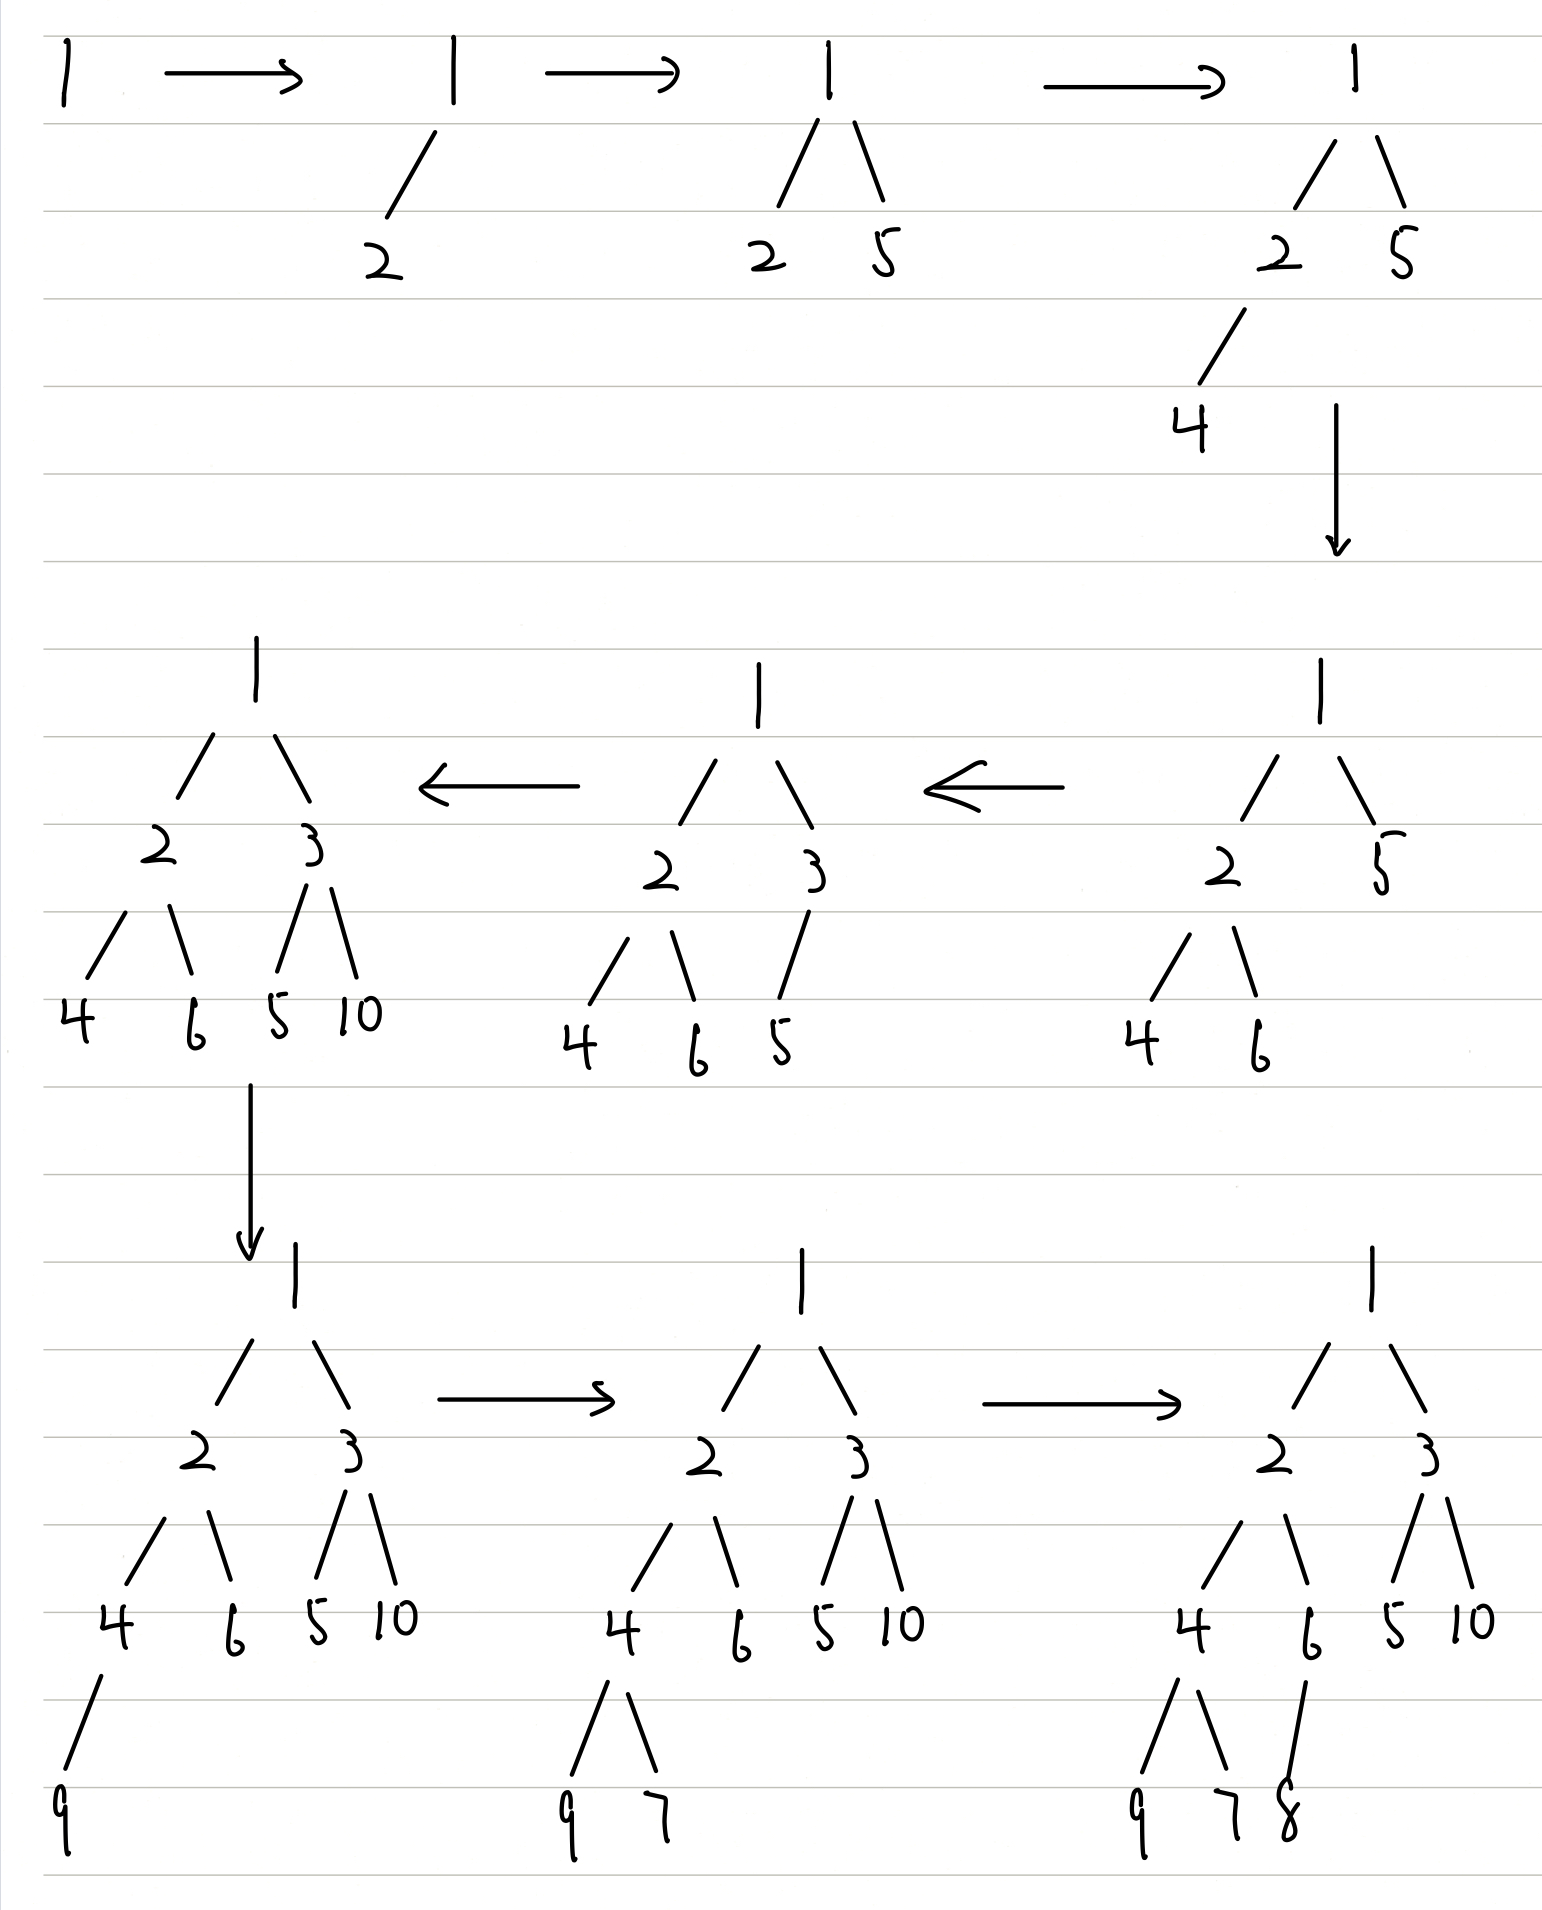
\includegraphics[width=0.9\columnwidth]{Q2.jpg}
\end{answer}

\begin{question}
\end{question}
%% Student: put your answer between the next two lines.
\begin{answer}
    Since this is a min-heap, to find out if there are at least $k$ items less than $x$, we only need to check the items in top $\lfloor \log k \rfloor + 1$ levels of the heap. Those items are the smallest items in the heap, and the number of those items, $k^\prime$ satisfies $k \leq k^\prime \leq 2k - 1$. Thus we only need to check at most $2k- 1$ items to determine whether there are at least $k$ items that are less than $x$.
\end{answer}

\begin{question}
\end{question}
%% Student: put your answer between the next two lines.
\begin{answer}
    \begin{enumerate}
    We use an AVL tree with some modifications to store those points.
        \begin{enumerate}
            \item
            In this AVL tree, the key is the coordinate of the points. Points with smaller $y$-coordinate should be on the left of the points with greater $y$-coordinate. If two points have same $y$-coordinate, then points with smaller $x$-coordinate should be on left.
            \item For each node, we store two values, the first value is the number of points that are in the lower left quadrant of the node's point. Since we insert points from left to right, this value would not change after the insertion.
            \item The second value is the total number of nodes that are on the left of this node plus one. It corresponds to the number of points that have a $y$-axis smaller or equal to current point's $y$-axis (including this point itself), but greater than $y$-axis of the point in \textbf{current node's parent node}. Its initial value after the insertion should always be $1$ since there are no nodes in the left right after the insertion.
            \item The two values in the first node is $(0, 1)$, since there is no point in the lower-left quadrant of this point, and there is only one point that have $y$-axis smaller or equal to the first point's $y$-axis (itself) and greater than its parent's $y$-axis (in this case, root node has no parent).
            \item Then during the insertion, we calculate the total number of points in the lower-left quadrant of the  point to be inserted by summing up second value of \textbf{all the nodes from which the insertion path head to its right child}. Besides, we increase the second value of \textbf{all the nodes from which the insertion path head to its left child} by one. It is easy to recalculate this second value for nodes that are involved in the rotation in constant time.
            \item After every insertion have been done, return first value of all the nodes. They are the numbers of points on the lower-left quadrant of each point.
            \item The following graph illustrates an example: \\
            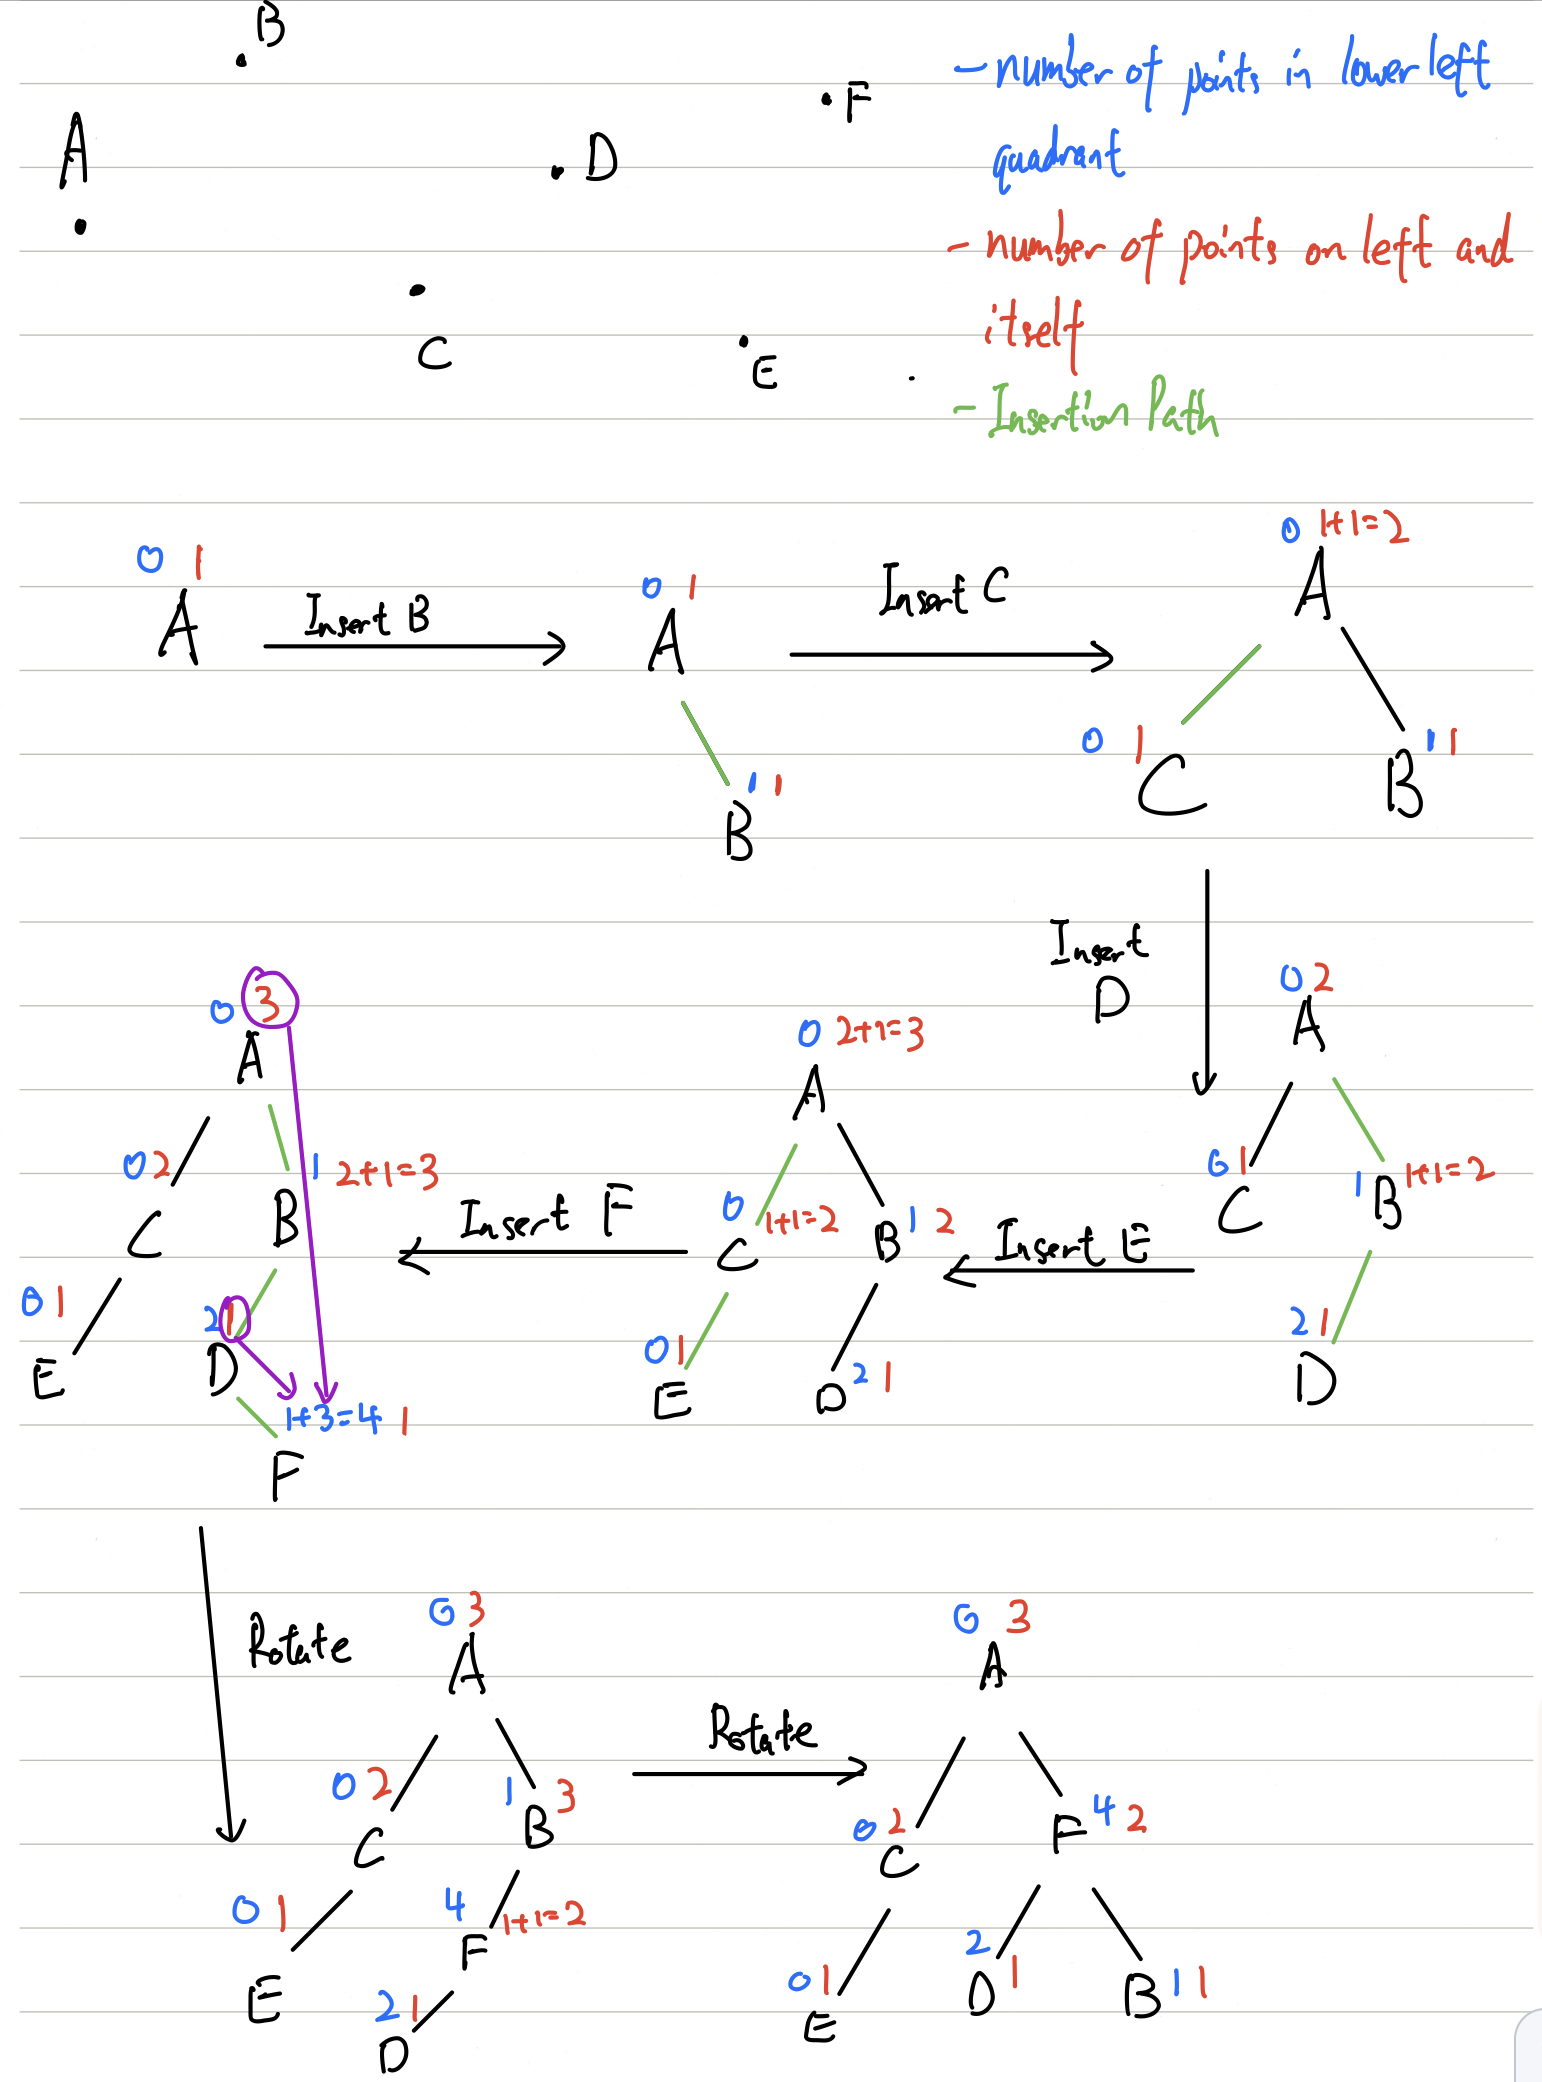
\includegraphics[width=0.8\columnwidth]{Q4.jpg}
            \item Each insertion and find operation takes $O(\log n)$, so the total time complexity is $O(n\log n)$
        \end{enumerate}
\end{enumerate}
\end{answer}

\begin{question}
\end{question}
%% Student: put your answer between the next two lines.
\begin{answer}
    \begin{enumerate}
        Setting up a DP table to solve this problem:
        \begin{enumerate}
            \item
            The DP table should have length $n$, and the $i$th element of the table is the length of the longest divisible subsequence ending at the $i$th element of the array.
            \item
            It is obvious that $DP \lbrack 1 \rbrack = 1$, and for following entries, $\displaystyle DP\lbrack k \rbrack = \max_{\substack{1 \leq i \leq k - 1 \\ a_i | a_k}} (DP\lbrack i \rbrack) + 1$. Finally, we return $DP \lbrack n \rbrack$
            \item
            To fill each entry, we need $O(n)$ time, and there are $n$ entries in total. Therefore, the total time complexity is $O(n^2)$
        \end{enumerate}
    \end{enumerate}
\end{answer}

\begin{question}
\end{question}
%% Student: put your answer between the next two lines.
\begin{answer}
    \begin{enumerate}
        Setting up a $2-dimesion$ DP table to solve this problem:
        \begin{enumerate}
            \item
            The DP table should have size of $n \times n$, and $DP \lbrack i \rbrack \lbrack j \rbrack$ is the minimum weight of path starting from $(1, 1)$ to $(i, j)$
            \item
            Let this matrix be $M$. $DP \lbrack 0 \rbrack \lbrack 0 \rbrack$ is $M_{00}$ ($0$ or $1$). Then we fill this table row by row, and for each row we fill that row from left to right. For each entry, $DP \lbrack i \rbrack \lbrack j \rbrack = \min (DP \lbrack i-1 \rbrack \lbrack j \rbrack, DP \lbrack i \rbrack \lbrack j-1 \rbrack) + M_{ij}$.
            \item
            To fill each entry, we need $O(n)$ time, and there are $n$ entries in total. Therefore, the total time complexity is $O(n^2)$
        \end{enumerate}
    \end{enumerate}
\end{answer}

\begin{question}
\end{question}
%% Student: put your answer between the next two lines.
\begin{answer}
    \begin{enumerate}
        Setting up a  DP table to solve this problem:
        \begin{enumerate}
            \item
            The DP table should have length $n$, and $DP \lbrack i \rbrack$ is the maximum value of $Cubesum(l, i)$, where $1 \leq l \leq i$.
            \item
            $DP \lbrack 1 \rbrack = Cubesum(1, 1) = a_1^3 $, and for following entries,
            \begin{equation*}
                DP \lbrack i \rbrack =
                \begin{cases}
                    a_i^3,\, DP \lbrack i-1 \rbrack < 0\\
                    DP \lbrack i-1 \rbrack + a_i^3,\, DP \lbrack i-1 \rbrack \geq 0
                \end{cases}
            \end{equation*}
            Finally, we return the maximum value in the table.
            \item
            To fill each entry, we need $O(1)$ time, and there are $n$ entries in total. Finding the maximum also takes $O(n)$ time. Therefore, the total time complexity is $O(n)$
        \end{enumerate}
    \end{enumerate}
\end{answer}

\begin{question}
\end{question}
%% Student: put your answer between the next two lines.
\begin{answer}
    \begin{enumerate}
        Setting up a DP table to solve this problem:
        \begin{enumerate}
            \item
            The DP table should have length $n$, and for each entry in the table, a tuple consists of three value is stored.\\
            $DP\lbrack i \rbrack \lbrack 1 \rbrack $ is the maximum length of stable subarray ending at $a_i$\\
            $DP\lbrack i \rbrack \lbrack 2 \rbrack $ is the \textbf{index of the first element in the last array of consecutive maximums} of that maximum-length subarray \\
            (For example, consider an almost stable array $1, 0, -1, 0, 0, 0$, $DP\lbrack 6 \rbrack \lbrack 1 \rbrack = 5$, and $DP\lbrack 6 \rbrack \lbrack 2 \rbrack = 4$, not $6$, because the index of the first $0$ in the last consecutive $0$s is $4$)\\
            Similarly, $DP\lbrack i \rbrack \lbrack 3 \rbrack $ is the \textbf{index of the first element in the last array of consecutive minimums} of that maximum-length subarray \\
            (In the previous case, $DP\lbrack 6 \rbrack \lbrack 3 \rbrack = 3$)
            \item
            $DP \lbrack 1 \rbrack = (1, 1, 1) $, and for following entries,
            \begin{equation*}
                \begin{aligned}
                    DP[i][1] &=
                    \begin{cases}
                        DP[i-1][1] + 1 &\text{ if } a_{DP[i-1][2]} - 2 < a_i < a_{DP[i-1][3]} + 2, \\
                        i - DP[i-1][2] + 1 &\text{ if } a_i \geq  a_{DP [i-1][3]} + 2\\
                        i - DP[i-1][3] + 1 &\text{ if } a_i \leq a_{DP[i-1][2]} - 2
                    \end{cases} \\
                    DP[i][2] &=
                    \begin{cases}
                        DP[i-1][2] &\text{ if } a_i = a_{DP[i-1][3]} \text{ or } (a_i > a_{DP[i-1][3]} \text{ and } a_i = a_{i-1})\\
                        i &\text{ if } a_i > a_{DP[i-1][3]} \text { and } a_i \neq a_{i-1}\\
                        DP[i-1][3]&\text{ if } a_i < a_{DP[i-1][3]}
                    \end{cases} \\
                    DP[i][3] &=
                    \begin{cases}
                        DP[i-1][3] &\text{ if } a_i = a_{DP[i-1][2]} \text{ or } (a_i < a_{DP[i-1][2]} \text{ and } a_i = a_{i-1})\\
                        i &\text{ if } a_i < a_{DP[i-1][2]} \text { and } a_i \neq a_{i-1}\\
                        DP[i-1][2]&\text{ if } a_i > a_{DP[i-1][2]}
                    \end{cases} \\
                \end{aligned}
            \end{equation*}
            Finally, we return $max(DP[i][1])$ in the table.
            \item
            The following table illustrate this update process:
            \begin{center}
            \begin{tabular}{ |c|c|c|c|c|c|c|c|c|c|c|c| }
                 \hline
                 index & 1 & 2 & 3 & 4 & 5 & 6 & 7 & 8 & 9 & 10 & 11 \\
                 \hline
                 value & 1 & 2 & 2 & 3 & 3 & 2 & 2 & 3 & 4 & 3 & 2 \\
                 \hline
                 length & 1 & 2 & 3 & 3 & 4 & 5 & 6 & 7 & 2 & 3 & 2 \\
                 last\,max & 1 & 2 & 2 & 4 & 4 & 4 & 4 & 8 & 9 & 9 & 10 \\
                 last\,min & 1 & 1 & 1 & 2 & 2 & 6 & 6 & 6 & 8 & 10 & 11 \\
                 \hline
            \end{tabular}
            \end{center}
            \item
            To fill each entry, we need $O(1)$ time, and there are $n$ entries in total. Finding the maximum also takes $O(n)$ time. Therefore, the total time complexity is $O(n)$
        \end{enumerate}
    \end{enumerate}
\end{answer}

\begin{question}
\end{question}
%% Student: put your answer between the next two lines.
\begin{answer}
    \begin{enumerate}
        \item Preordering the tree, we could convert it to
        \begin{equation*}
            [(C,5), (E,4), (A,10), (D,20), (B,2)]
        \end{equation*}
    \end{enumerate}
\end{answer}

\end{document}
\endinput
%%
%% End of file `ps2.ans.tex'.
